\subsection{NEIGHBOURHOODS}

DEFINITION 4. Let X be a topological space and A any subset of X. A neighbourhood of A is any subset of X which contains an open set containing A. The neighbourhoods of a subset \(\{x\}\) consisting of a single point are also called neighbourhoods of the point x.

It is clear that every neighbourhood of a subset A of X is also a neighbourhood of each subset \(B \subset A\) ; in particular, it is a neighbourhood of each point of A. Conversely, suppose A is a neighbourhood of each of the points of a set B, and let U be the union of the open sets contained in A; then \(U \subset A\) , and since each point of B belongs to an open set contained in A, we have \(B \subset U\) ; but U is open by virtue of \((\mathrm{O}_{\mathrm{I}})\) , hence A is a neighbourhood of B. In particular:

PROPOSITION 1. A set is a neighbourhood of each of its points if and only if it is open.

The everyday sense of the word ``neighbourhood'' is such that many of the properties which involve the mathematical idea of neighbourhood appear as the mathematical expression of intuitive properties; the choice of this term thus has the advantage of making the language more expressive. For this purpose it is also permissible to use the expressions ``sufficiently near'' and ``as near as we please'' in some statements. For example, Proposition 1 can be stated in the following form: a set A is open if and only if, for each \(x \in A\) , all the points sufficiently near x belong to A. More generally, we shall say that a property holds for all points sufficiently near a point x, if it holds at all points of some neighbourhood of x.

Let us denote by \(\mathfrak{B}(x)\) the set of all neighbourhoods of \(x\) . The sets \(\mathfrak{B}(x)\) have the following properties:

\((\mathbf{V}_{\mathbf{I}})\) Every subset of \(\mathbf{X}\) which contains a set belonging to \(\mathfrak{B}(x)\) itself belongs to \(\mathfrak{B}(x)\) .

\((V_{II})\) Every finite intersection of sets of \(\mathfrak{B}(x)\) belongs to \(\mathfrak{B}(x)\) .

\((V_{\mathrm{III}})\) The element \(x\) is in every set of \(\mathfrak{B}(x)\) .

Indeed, these three properties are immediate consequences of Definition 4 and axiom (O \(_{II}\) ).

\((V_{IV})\) If V belongs to \(\mathfrak{B}(x)\) , then there is a set W belonging to \(\mathfrak{B}(x)\) such that, for each \(y \in W\) , V belongs to \(\mathfrak{B}(y)\) .

By Proposition 1, we may take W to be any open set which contains x and is contained in V.

This property may be expressed in the form that a neighbourhood of x is also a neighbourhood of all points sufficiently near to x.

These four properties of the sets \(\mathfrak{B}(x)\) are characteristic. To be precise, we have:

PROPOSITION 2. If to each element \(x\) of a set \(\mathbf{X}\) there corresponds a set \(\mathfrak{B}(x)\) of subsets of \(\mathbf{X}\) such that the properties \((\mathbf{V}_{\mathbf{I}}), (\mathbf{V}_{\mathbf{II}}), (\mathbf{V}_{\mathbf{III}})\) and \((\mathbf{V}_{\mathbf{IV}})\) are satisfied, then there is a unique topological structure on \(\mathbf{X}\) such that, for each \(x \in \mathbf{X}\) , \(\mathfrak{B}(x)\) is the set of neighbourhoods of \(x\) in this topology.

By Proposition 1, if there is a topology on X satisfying these conditions, the set of open sets for this topology is necessarily the set \(\mathfrak{D}\) of subsets A of X such that for each \(x \in \mathbf{A}\) we have \(\mathbf{A} \in \mathfrak{B}(x)\) ; hence the uniqueness of this topology if it exists.

The set \(\mathfrak{D}\) certainly satisfies axioms \((\mathrm{O_I})\) and \((\mathrm{O_{II}})\) : for \((\mathrm{O_I})\) , this follows immediately from \((\mathrm{V_I})\) , and for \((\mathrm{O_{II}})\) , from \((\mathrm{V_{II}})\) . It remains to show that, in the topology defined by \(\mathfrak{D}\) , \(\mathfrak{B}(x)\) is the set of neighbourhoods of \(x\) for each \(x \in \mathbf{X}\) . It follows from \((\mathbf{V}_{\mathbf{I}})\) that every neighbourhood of \(x\) belongs to \(\mathfrak{B}(x)\) . Conversely, let \(\mathbf{V}\) be a set belonging to \(\mathfrak{B}(x)\) , and let \(\mathbf{U}\) be the set of points \(y \in \mathbf{X}\) such that \(\mathbf{V} \in \mathfrak{B}(y)\) ; if we can show that \(x \in \mathbf{U}\) , \(\mathbf{U} \subset \mathbf{V}\) and \(\mathbf{U} \in \mathfrak{D}\) , then the proof will be complete. We have \(x \in \mathbf{U}\) since \(\mathbf{V} \in \mathfrak{B}(x)\) ; also \(\mathbf{U} \subset \mathbf{V}\) , for every point \(y \in \mathbf{U}\) belongs to \(\mathbf{V}\) by reason of \((\mathbf{V}_{\mathbf{III}})\) and the hypothesis \(\mathbf{V} \in \mathfrak{B}(y)\) . It remains to show that \(\mathbf{U} \in \mathfrak{D}\) , i.e.~that \(\mathbf{U} \in \mathfrak{B}(y)\) for each \(y \in \mathbf{U}\) ; now (Fig. 1) if \(y \in \mathbf{U}\) then by \((\mathbf{V}_{\mathbf{IV}})\) there is a set \(\mathbf{W}\) such that for each \(z \in \mathbf{W}\) we have \(\mathbf{V} \in \mathfrak{B}(z)\) ; since \(\mathbf{V} \in \mathfrak{B}(z)\) means that \(z \in \mathbf{U}\) , it follows that \(\mathbf{W} \subset \mathbf{U}\) , and therefore, by \((\mathbf{V}_{\mathbf{I}})\) , that \(\mathbf{U} \in \mathfrak{B}(y)\) . Q.E.D.

\pandocbounded{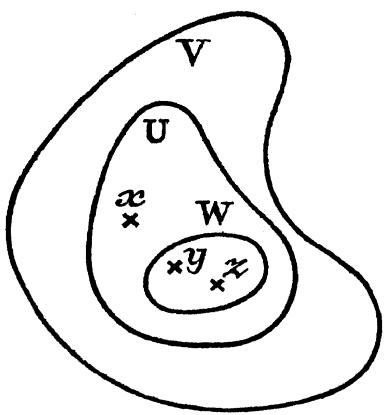
\includegraphics[keepaspectratio]{images/part001_56c83e78.jpg}}\\
Figure 1.

Proposition 2 shows that a topology on X can be defined by means of the sets \(\mathfrak{B}(x)\) of neighbourhoods of points of X, subject only to the axioms \((\mathrm{V}_{\mathrm{I}})\) , \((\mathrm{V}_{\mathrm{II}})\) , \((\mathrm{V}_{\mathrm{III}})\) and \((\mathrm{V}_{\mathrm{IV}})\) .

Example. We may define a topology on the set \(\mathbf{Q}\) of rational numbers by taking for open sets all unions of bounded open intervals; the set of these subsets certainly satisfies \((\mathrm{O}_{\mathbf{I}})\) , and to see that it satisfies \((\mathrm{O}_{\mathbf{II}})\) it is enough to remark that if the intersection of two open intervals \(]a, b[\) and \(]c, d[\) is not empty, then it is the interval \(]\alpha, \beta[\) , where \(\alpha = \sup (a, c)\) and \(\beta = \inf (b, d)\) . We get the same topology by defining for each \(x \in \mathbf{Q}\) the set \(\mathfrak{B}(x)\) of neighbourhoods of \(x\) to be the set of subsets containing an open interval to which \(x\) belongs. The topological space obtained by assigning this topology to \(\mathbf{Q}\) is called the rational line (cf.~Chapter IV, § 1, no. 2). Notice that in this space every open interval is an open set. * We can define a topology on the set \(\mathbf{R}\) of real numbers in the same way; \(\mathbf{R}\) with this topology is called the real line (cf.~§ 2, Exercise 5 and Chapter IV, § 1, no. 3). *

